\section{Flat Combining}

At the most basic level, the concept of flat combining is about enabling cooperation among threads rather than contention. The benefits can be broken down into three components: improved locality, reduced synchronization, and data-structure-specific optimization. We will explore how this works in a traditional shared-memory system, and then describe how the same concepts can be applied to distributed memory.

% Flat combining allows threads to cooperate when accessing a synchronized shared data structure to get greater overall throughput than even each of them operating serially. However, the same delegation mechanism can be reused in any data structure protected by a single global lock. 

\subsection{Physically shared memory}

\begin{figure}[t]
  \centering
  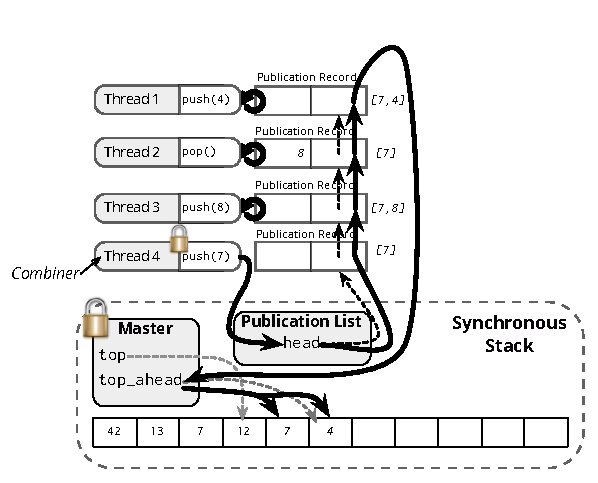
\includegraphics[width=0.42\textwidth]{figs/fc_shared_mem.pdf}
  \caption{\emph{Flat combining in shared memory.}
    To access the shared stack, each thread adds its request to the publication list (1). Thread 4 acquires the stack's lock and becomes the combiner (2), while the remaining threads spin waiting for their request to be satisfied. The combiner walks the publication list from the head, matching up Thread 3's push with Thread 2's pop on its own private stack (3). The two remaining pushes are added to the top of the shared stack (4). Finally, the top is updated, and Thread 4 releases the lock and continues its normal execution.
  }
  \label{fig:fc_shared_mem}
\end{figure}

% One of the issues with shared data structures in a shared-memory multicore is that threads executing on different cores will force the hottest parts of the data structure to thrash between their caches. Having a single thread do all of the operations on the data structure allows it to keep everything in its cache.

% Improving locality in a shared-memory multicore is achieved by 
% Having a single thread bound to a particular core do a string of accesses trivially results in a lower cache miss rate than having multiple threads on multiple cores bring the data structure into cache each in turn.

% Careful engineering must be employed to implement a mechanism for cooperation that does not introduce the same synchronization issues as the original contended data structure.

Simply by delegating work to another core, locality is improved and synchronization is reduced.
Consider the shared synchronous stack shown in Figure~\ref{fig:fc_shared_mem}, with pre-allocated storage and a \texttt{top} pointer protected by a lock. Without flat combining, whenever a thread attempts to push something on the stack, it must acquire the lock, put its value into the storage array, bump the top, and then release the lock. When many threads contend for the lock, all but one will fail and have to retry. Each attempt forces an expensive memory fence and consumes bandwidth, and as the number of threads increases, the fraction of successes plummets. Under flat combining, instead, threads add requests to a \emph{publication list}. They each try to acquire the lock, and the one that succeeds becomes the combiner. Instead of retrying, the rest spin on their request waiting for it to be filled. The combiner walks the publication list, performs all of the requests, and when done, releases the lock. This allows the one thread to keep the data structure in cache, reducing thrashing between threads on different cores. It also greatly reduces contention on the lock, but introduces a new point of synchronization---adding to the publication list. However, if a thread performs multiple operations, it can leave its publication record in the list and amortize the synchronization cost. This publication list mechanism can be re-used in other data structures, saving each from needing to implement its own clever synchronization.

The above example of delegation is compelling in itself. However, the crux of prior work is that data structure-specific optimization can be done to perform the combined operations more efficiently.
As the combiner walks the publication list, it merges each non-empty publication record into a combined operation. In the case of the stack example shown in Figure~\ref{fig:fc_shared_mem}, as it walks the list, Thread 4 keeps track of the operations on its own temporary stack. When it encounters Thread 2's pop, it recognizes that it can satisfy that pop immediately with the push it just processed from Thread 3, so it fills both of their records and allows them to proceed. After traversing the rest of the publication list, the thread applies the combined operation to the actual data structure, in this case, the two unmatched pushes are added to the top of the stack.
In the case of the stack, combining came in the form of matched pushes and pops, but many data structures have other ways in which operations can be matched.

\subsection{Grappa}

% \begin{figure*}[t]
%   \begin{subfigure}[b]{0.38\textwidth}
\begin{figure}[t]
    \centering
    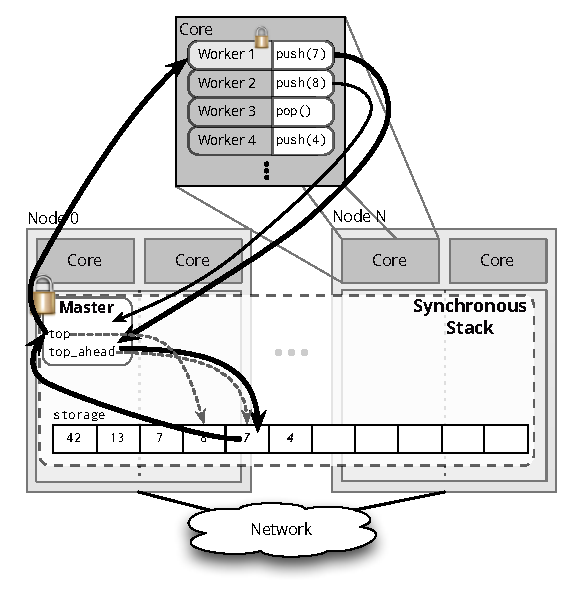
\includegraphics[width=0.40\textwidth]{figs/stack_nofc.pdf}
    \caption{\emph{Stack without combining.}
      To do its push, Worker 1 sends a message to synchronize with the master on Core 0 (1), which sends another message to write the value to the top of the stack (2), bumps the synchronized \texttt{top} pointer (3), and finally continues. Worker 2, and workers on other cores, must block at the master and wait for Worker 1 to complete its push before doing their operations (4).
    }
    \label{fig:stacknofc}
  % \end{subfigure}%
  % \hspace{0.12\textwidth}
\end{figure}
\begin{figure}
  % \begin{subfigure}[b]{0.38\textwidth}
    \centering
    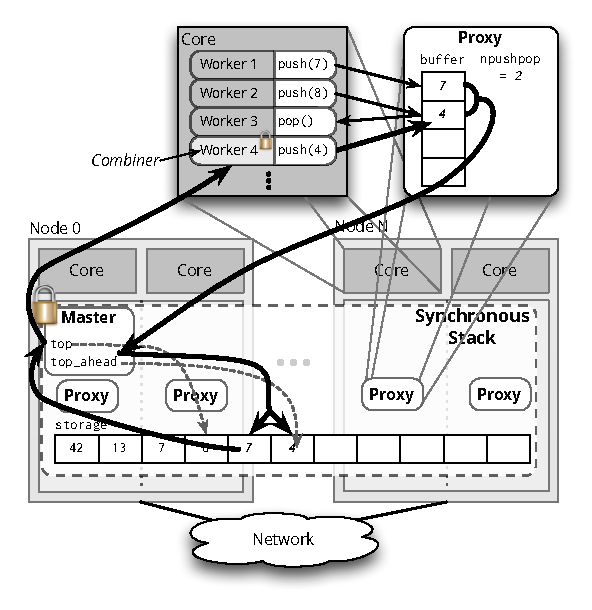
\includegraphics[width=0.42\textwidth]{figs/stack_fc.pdf}
    \caption{\emph{Stack with distributed combining.}
      Worker 3's pop matches with Worker 2's push, requiring no global communication (1). After combining locally, Worker 1 and 4's pushes remain, so Worker 4 becomes the core's combiner (2), sends a message to synchronize with the master (3), adds both new values to global stack (4), bumps the top pointer and releases the lock on master (5), and finally wakes Worker 1 (6).
    }
    \label{fig:stackfc}
  % \end{subfigure}
\end{figure}
  % \caption{\emph{Global stack in Grappa} with and without \emph{flat combining}.}
  % \label{fig:stack}
% \end{figure*}

In a PGAS setting, and in Grappa in particular, the cost of global synchronization and the amount of concurrency is even greater than in shared memory. With thousands of workers per core, in a reasonably sized cluster there are easily millions of workers. This presents an opportunity for flat combining to pay off greatly, but also poses new challenges.

% a number of different choices are made when implementing flat combining. Because memory is physically distributed, locality must be made explicit. In addition, in Grappa there are orders of magnitude more concurrent threads (``workers'') accessing shared data structures. Typically around a thousand are needed per core to tolerate the latency of remote operations, so in a cluster of machines, there are easily millions of workers. Therefore, a different scheme for managing many threads is necessary.

To illustrate how flat combining can be applied to Grappa, we must first describe what a global data structure looks like. Figure~\ref{fig:stacknofc} shows a simple PGAS translation of the shared-memory stack from earlier. A storage array is allocated in the global heap, so its elements are striped across all the cores in the system. One core is designated the \emph{master} to enforce global synchronization, and holds the elements of the data structure that all concurrent accessors must agree on, in this case, the \texttt{top} pointer.

All tasks accessing the stack hold a \texttt{GlobalAddress} to the master object, and invoke custom \emph{delegate methods} that, like the \texttt{read} delegate described earlier, block the task until complete. Example code to do a \texttt{push} is shown in Figure~\ref{fig:push}. The task must send a message to the master to acquire the lock. If successful, it follows the \texttt{top} pointer, writes its new value to the end of the stack, returns to bump the \texttt{top} pointer and release the lock, and finally sends a message back to wake the calling worker. All others block at the first message until the lock is released. Grappa's user-level threading allows requests to block without consuming compute resources. However, all workers on each core perform this synchronization and serialize on a single core, causing that core to become the bottleneck.

\paragraph{Centralized Combining.}
A first thought might be to directly apply the idea of flat combining to the serialization at the \emph{master}. The worker that acquires the lock can walk through the requests of all the other workers waiting to acquire the lock and combine them. In the case of the Stack, this would mean matching pushes and pops, applying the remainder, and sending messages back to all remote workers with results, before starting another round of combining. This approach reduces traffic to the data structure storage, but a single core must still process every request, so it cannot scale if every other core is generating requests at the same rate.

\paragraph{Distributed Combining.}
Instead of all workers sending independent synchronization messages and putting the burden all on one core, each core can instead do its own combining first then synchronize with the master in bulk.
Distributing the combining to each core allows the majority of the work to be performed in parallel and without communication.
% As with shared-memory combining, distributed combining improves locality, reduces the amount of global synchronization, and allows operations to be composed in data structure-specific ways for even greater performance.

% In a way, Grappa's automatic message aggregation is already trying to reduce synchronization traffic; however, the generic mechanism for serializing and packing has a cost, and in the end, the operations must still serialize on the master.
% Flat combining is about ``teaching'' it how to more efficiently perform many operations remotely in certain special cases.

In distributed flat-combining, each core builds its own publication list to track all the operations waiting to be committed to the global data structure.
In Grappa, for each global data structure, a local \emph{proxy} object is allocated from the core-local heap to intercept requests.
Conceptually, workers add their requests to a local publication list in the proxy, one is chosen to do the combining, and the rest block until their request is satisfied.
However, because Grappa's scheduler is non-preemptive, each worker has atomicity ``for free'' until it performs a blocking operation (such as communication).
This means that an explicit publication list with clever synchronization is unnecessary.
Instead, workers merge their operations directly into the local proxy, and 
% block if unable to satisfy their requests immediately.
block, except in restricted cases where they are able to satisfy their requirements immediately without violating ordering rules for consistency (discussed in the next section).
The proxy structure is chosen to be able to compactly aggregate operations and efficiently perform matching in cases where it is allowed. Figure~\ref{fig:stackfc} shows how pushes and pops are matched on the proxy's local stack.

After all local combining has been done, one requesting worker on the core is chosen to commit the combined operation globally. In Figure~\ref{fig:stackfc}, Worker 4 becomes the combiner and performs much the same synchronization as in the uncombined case, but is able to push multiple elements with one synchronization. The global lock must still be acquired, so concurrent combined requests (from different cores) must block and serialize on the master, but the granularity of global synchronization is coarser, reducing actual serialization.

\paragraph{Memory Consistency Model.}
\label{sec:memory-model}
In the context of Grappa, sequential consistency guarantees that within a
task, operations will be in task order and that all tasks will observe the
same global order.
The Grappa memory model is essentially the same as the C++ memory
model~\cite{boehm:drf0,N2480,N2800}, guaranteeing sequential
consistency for data-race free programs. To be conservative, delegate
operations block the calling worker until they have become globally visible,
ensuring they can be used for synchronization. As such, delegate operations
within a task are guaranteed to be globally visible in program order and all
tasks observe the same global order.
Operations on synchronized data structures must provide the same guarantees.
Because it is not immediately obvious
that this distributed version of flat combining preserves sequential
consistency, we now argue why it does.

To preserve linearizability for flat-combined operations, they must obey a consistent global order.
First of all, the execution of local combined operations must be serializable;
this is unchanged from shared-memory flat-combining, and is trivially true due to the atomicity enabled by cooperative multithreading.
When combined operations are applied globally, they are serialized at a particular core that owns the synchronization (the \emph{master} core for the Stack).
Whenever a global commit starts, a fresh combiner must be created for subsequent operations to use. If they were to use the old combiner's state to satisfy requests locally, it would violate global ordering because the local object would not reflect other cores' updates.
% This guarantees, for example, that destructive operations only happen once (i.e., a worker cannot locally pop the same value that another core's combined operation does).
% haven't discussed queue, set, or map yet...
%(the ``master'' core for the Queue and Stack, or the corresponding hash cell for the Set and Map). The global order, then, is essentially the concatenation of the cores' sequential orders.
For this serial ``concatenation'' of serialized batches to be valid, the order observed by workers during local combining must be the same as what can be observed globally as operations are committed.

In the case of a stack or queue, this guarantee comes from applying a batch of push or pop operations atomically in a contiguous block on the global data structure.
% Centralized combining preserves this by only allowing updates to proceed when they will not conflict and blocking a batch of operations until all have completed.
Matching pushes and pops locally for the Stack is one exception to the rule that operations must block until globally committed. Because a pop ``destroys'' the corresponding push, these operations together are independent of all others and can conceptually be placed anywhere in a global order. It is trivial to respect program order with this placement, so they can be safely matched locally.

Combining set and map operations expose more nuances in the consistency guarantees.
Insert and lookup operations performed by different tasks are inherently unordered unless synchronized externally.
Therefore, a batch of these operations can be committed globally in parallel, since they are guaranteed not to conflict with each other.
Note that if an insert finds that its key is already in the combiner object, it does not need to send its own message. However, it must still block until that insert is done to ensure that a subsequent operation it performs cannot be reordered with it, preserving program order.
% providing the same guarantee as all other delegate operations. 
% This ensures that if one wanted to use the insert to signal synchronization, it is guaranteed to have been committed globally before the task continues.

Similarly, lookups can piggy-back on other lookups of the same key.
Using intuition from store/write buffers in modern processors, it is tempting to allow a lookup to be satisfied locally by inspecting outstanding inserts.
However, this allows the local order in which keys were inserted to be observed.
If this is allowed, then to preserve SC, that same order must be respected globally, forcing each batch to commit atomically with respect to other cores' batches. Enforcing this is prohibitively expensive, so a cheaper solution is chosen: lookups must get their values from the global data structure, so batches can be performed in parallel.

These requirements only guarantee linearizability of operations on a single data structure. To guarantee sequential consistency with respect to all accesses, data-race freedom must be guaranteed by the program, as in the C++ memory model for shared memory.

\section{Grappa FC Framework}
To leverage the flat-combining paradigm in Grappa, we implemented a generic framework to improve performance for a number of global data structures. The FC framework handles the common problems of managing the combiners, handling worker wake-ups, and maintaining progress. When hooking into the framework, each data structure need only define how to combine operations and globally commit them.

As mentioned before, the Grappa FC framework takes a different approach than the original flat-combining work for expressing how operations combine.
% As mentioned before, the local \emph{publication list} is trivial to access atomically in Grappa's cooperative scheduling.
% Instead, in the Grappa FC Framework, 
For each global structure instance, a \emph{proxy} object is created on each core and each worker merges its request into that structure before blocking or becoming the combiner.
Each global data structure must define a \emph{proxy} that has \emph{state} to track combined requests, \emph{methods} to add new requests, and a way to \emph{sync} the state globally.
% \begin{enumerate}
%   \item A local \emph{proxy} data structure for tracking combined requests.
%   \item \emph{Combining methods} that operate on the local proxy.
%   \item A \emph{sync} method that globally commits the proxy's state.
% \end{enumerate}
An example proxy declaration for the GlobalStack is shown in Figure~\ref{fig:push}.

\begin{figure}[t]
\centering
\begin{lstlisting}[style=grappa]
// Global master state
class GlobalStack {
  GlobalAddress<T> top;
  Grappa::Mutex lock;
};
// Push *without* combining
void push(GlobalAddress<GlobalStack> master, T e){
  // from stack's master core, perform write to top and increment atomically
  delegate::call(master.core(), [master,e]{
    master->lock.acquire();
    delegate::write(master->top, e);
    master->top++;
    master->lock.release();
  }); // blocks until response arrives
}
// Definition of proxy
class GlobalStackProxy : Grappa::FCProxy {
  GlobalAddress<GlobalStack> master;
  // Local state for tracking requests
  T  pushed_values[1024];
  T* popped_results[1024];
  int npush, npop;

  // Combining Methods 
  void push(T val);
  T pop();
  
  // Global sync (called by FC framework)
  void sync() override {
    if (npush > 0) {
      // on master: acquire lock, return top ptr
      auto top = delegate::call(master.core(),[=]{
        master->lock.acquire();
        return master->top;
      });
      // copy values to top of stack
      Grappa::memcpy(top, pushed_values, npush);
      // bump top and release lock
      delegate::call(master.core(),[master,npush]{
        master->top += npush;
        master->lock.release();
      });
    } else if (npop > 0) {} // elided for space...
  }
};
\end{lstlisting}
\caption{Snippet of code from GlobalStack.
% Note how the combined \texttt{push} resembles the uncombined version but for multiple elements.
}
\label{fig:push}
\end{figure}

% The FC framework does the bookkeeping to block and wake workers, deliver results, manage when to synchronize, and choose the combiner.
The FC framework is responsible for ensuring that all of the combined operations eventually get committed. There are a number of ways progress could be guaranteed, but one of the simplest is to ensure that as long as there are any outstanding requests, at least one worker is committing a combined operation.
When that combined operation finishes, if there are still outstanding requests that have built up in the meantime, another blocked worker is chosen to do another combined synchronization.

% % left out for space
% One could imagine other synchronization policies that would ensure progress but allow more combining to occur before synchronizing. For instance, local combining could continue until all workers are blocked. However, this would require the flat-combining framework to track the activity of the workers on a core, and additionally would add latency unless the system saved enough active workers to tolerate the latency of the global commit action. As it is, the one-in-flight policy implemented performs well, and does not require any coupling with the Grappa scheduler. Exploration of other policies is left for future work.

While a combining operation is in flight, new requests continue to accumulate. The framework transparently wraps the proxy object so when one \texttt{sync} starts, it can direct requests to a fresh combiner.
This is done by hiding instances of proxy objects behind a C++ smart-pointer-like object which provides the pointer to the current combiner, and whenever it detects that it should send, allocates a new combiner and points subsequent references to that.
% Requests cannot be combined with others that have been committed or are currently being committed; we refer readers to Section~\ref{sec:memory-model} for why this must be so.
% Updates cannot be added to combiners that are in the process of being committed and must start out fresh each time; it would be unsound for them to ``remember'' the previous updates and attempt to combine locally with them. 

\subsection{Global Stack and Queue}
Figure~\ref{fig:push} shows an excerpt from the definition of the proxy object for the Grappa GlobalStack. The proxy tracks pushes in the \texttt{pushed\_values} array. When \texttt{pop} is called, if there are pushes, it immediately takes the top value and wakes the last pusher. Otherwise, it adds a pointer to a location on its stack where the \texttt{sync} operation will write the result. Because of local matching, when a Stack proxy is synchronized, it will have either all pops or all pushes, which makes the implementation of sync straightforward. Note that the operation to synchronize a batch of pushes looks almost identical to the code to do a single push from Figure~\ref{fig:push}.

The GlobalQueue has nearly the same implementation as the stack, but is unable to match locally.
%, so \texttt{sync} first commits the pushes, then the pops.

\subsection{Global Set and Map}
The Grappa GlobalSet uses a simple chaining design, implemented with a global array of cells (allocated from the global heap), which are partitioned evenly among all the cores, and indexed with a hash function. Our flat-combining version supports both \texttt{insert} and \texttt{lookup}. To track all of the keys waiting to be inserted, we use the hash set implementation from the C++11 standard library (\texttt{std::unordered\_set}). As with pops, lookups must provide pointers to stack space where results should be put, which is done with a hash map (again from the C++ standard library) from keys to lists of pointers. As discussed in Section~\ref{sec:memory-model}, matching lookups with inserts locally would force a particular sequential order. Instead, we only allow matching inserts with inserts and lookups with lookups, allowing \texttt{sync} to simply issue all inserts and lookups in parallel and block until all have completed.

Our implementation of the GlobalMap matches that of the Set but of course stores values.
 % This does not change the requirements of the proxy except that the return values of lookups must be a copy of the value rather than just a boolean.

